\chapter{Implementace}
Tato kapitola popisuje implementaci knihovny ATTYC (\textit{ATom TYpe Classification}), která přiřazuje atomům molekulového souboru atomové typy na základě zvolené vlastnosti atomu. Kromě klasifikátoru \verb|peptide|, který je určen výhradně pro formát PDB, lze zbylé klasifikátory libovolně použít pro formát PDB i SDF. Knihovna je implementována v~jazyce Python ver. 3.7 a obsahuje následující soubory:
% Pro formát PDB je určen klasifikátor \verb|peptide|, klasifikátory \verb|hbo|, \verb|hybrid|, \verb|part-|\\\verb|ners| a \verb|substruct| se vztahují k formátu  SDF. Knihovna je implementována v jazyce Python ver. 3.7 a obsahuje následující soubory:

\vspace{0.4cm}
\noindent \hangpara{1.5cm}{1} \textbf{\_\_init\_\_.py} obsahuje funkci \verb|classify_atoms(input_file, classifier)|\footnote{Argumenty \texttt{file\_output} a \texttt{screen\_output} jsou pro větší přehlednost v textu vynechány.}
spouštějící klasifikaci atomů molekulové sady za uži\-tí zvoleného klasifikátoru

\medskip
\noindent \textbf{classifier.py} definuje rozhraní pro klasifikátory implementované v adresáři \textbf{\textbackslash classifiers}

\medskip
\noindent \textbf{exceptions.py} definuje výjimky (potomky třídy Exception) pro řízení běhu programu

\medskip
\noindent \hangpara{1.5cm}{1}\textbf{io.py} zpracovává všechny vstupy a výstupy (I/O) programu včetně kontroly vstupních argumentů 

\medskip
\noindent \hangpara{1.5cm}{1}\textbf{PDB\_atom\_types.txt} obsahuje názvy atomů aminokyselin definovaných nomenklaturou IUPAC a přiřazené atomové typy pro klasifikaci atomů v PDB souborech

\medskip
\noindent \hangpara{1.5cm}{1}\textbf{SMARTS\_atom\_types.txt} obsahuje SMARTS výrazy a odpovídající atomové typy pro vyhledání specifických strukturních motivů a funkčních skupin 
% (viz sekci \ref{substruct})

\medskip
\noindent\textbf{\textbackslash classifiers} obsahuje klasifikátory, které rozdělují atomy do atomových typů na základě:

\medskip
\textbf{\_\_init\_\_.py}

\vspace{0.01cm}
\textbf{hbo.py} nejvyššího řádu vazby (\textit{highest bond order})

\vspace{0.01cm}
\textbf{hybrid.py} hybridizace

\vspace{0.01cm}
\textbf{partners.py}\ vazebných partnerů

\vspace{0.01cm}
\textbf{peptide.py} pozice atomu v rámci aminokyseliny
    
\vspace{0.01cm}
\textbf{substruct.py} příslušnosti ke strukturnímu motivu nebo funkční skupině

\bigskip
Výstup knihovny ATTYC je specifikován argumenty \verb|file_output| a \verb|screen_output| funkce \verb|classify_atoms(...)|. Pokud má argument \verb|file_output| hodnotu \verb|True|, jsou přiřazené atomové typy molekul zapsány do textového souboru. V případě použití argumentu \verb|screen_output| je na standardní výstup vypsána statistika přiřazených atomových typů.


\section{Spuštění klasifikace}
% \texttt{classify\_atoms(input\_file, classifier)}
Klasifikace atomů do atomových typů vstupního molekulového souboru je spuštěna voláním fun\-kce \verb|classify_atoms(input_file, classifier)|, která je 
implementována v modulu \textbf{\_\_init\_\_.py} v adresáři \textbf{attyc}. Příkaz \verb|attyc.classify_atoms(input_fi|\\ \verb|le, classifier)| spouští klasifikaci atomů z libovolného programu v jazyce Python, do kterého byla integrována knihovna ATTYC. Pro spuštění klasifikace je nutné do interpretu Pythonu daného programu nainstalovat knihovnu RDKit. 

V rámci funkce \verb|classify_atoms(input_file, classifier)| je kontrolována e\-xistence vstupního molekulového souboru a zvoleného klasifikátoru. Pokud je klasifikátor (tzn. podtřída třídy Classifier) implementován v adresáři \textbf{\textbackslash classifiers} a je povolen pro daný molekulový formát, je vytvořena jeho instance. Tato instance přiřazuje atomům v molekulové sadě odpovídající atomový typ.

%voláním metody \verb|get_atom_types(molecule)|, která je volána skrze metodu \verb|classify_atoms_by_classifier(moleculeset, is_pdb)| třídy Classifier. Metoda \verb|get_atom_types(molecule)| je abstraktní metodou třídy Classifer a je implementována všemi podtřídami třídy Classifier.

\section{Dědičnost třídy Classifier}
Třída Classifier definuje rozhraní pro podtřídy definované v modulech v adresáři \textbf{\textbackslash classifiers}. %Všechny podtřídy třídy Classifier obsahují atribut \verb|assigned_atom_types|, do~kterého ukládají přiřazené atomové typy, a atribut \verb|name|. 
Kromě getterů atribu\-tů \verb|assigned_atom_types| a \verb|name| dědí podtřídy metodu \verb|classify_atoms_by_classifier(moleculeset, is_pdb)|. Ta\-to metoda volá abstra\-ktní metodu \verb|get_atom_types(molecule)|, kterou každá podtřída třídy Classifier implementuje. Podtřídy, které představují klasifikátory \verb|substruct| a \verb|peptide|, obsahují kromě výše uvedených atributů také atributy pro uložení dat z externích souborů potřebných pro klasifikaci atomů.

Každý modul v adresáři \textbf{\textbackslash classifiers} obsahuje právě jednu podtřídu třídy Classifier (dále jen 'klasifikátor'). Implementace třídy Classifier je na klasifikátorech definovaných v tomto adresáři nezávislá, moduly v adresáři spolu nijak neinteragují. Knihovna je tak snadno rozšiřitelná o další libovolné klasifikátory. 

\bigskip
\begin{figure}[h]
    \centering
    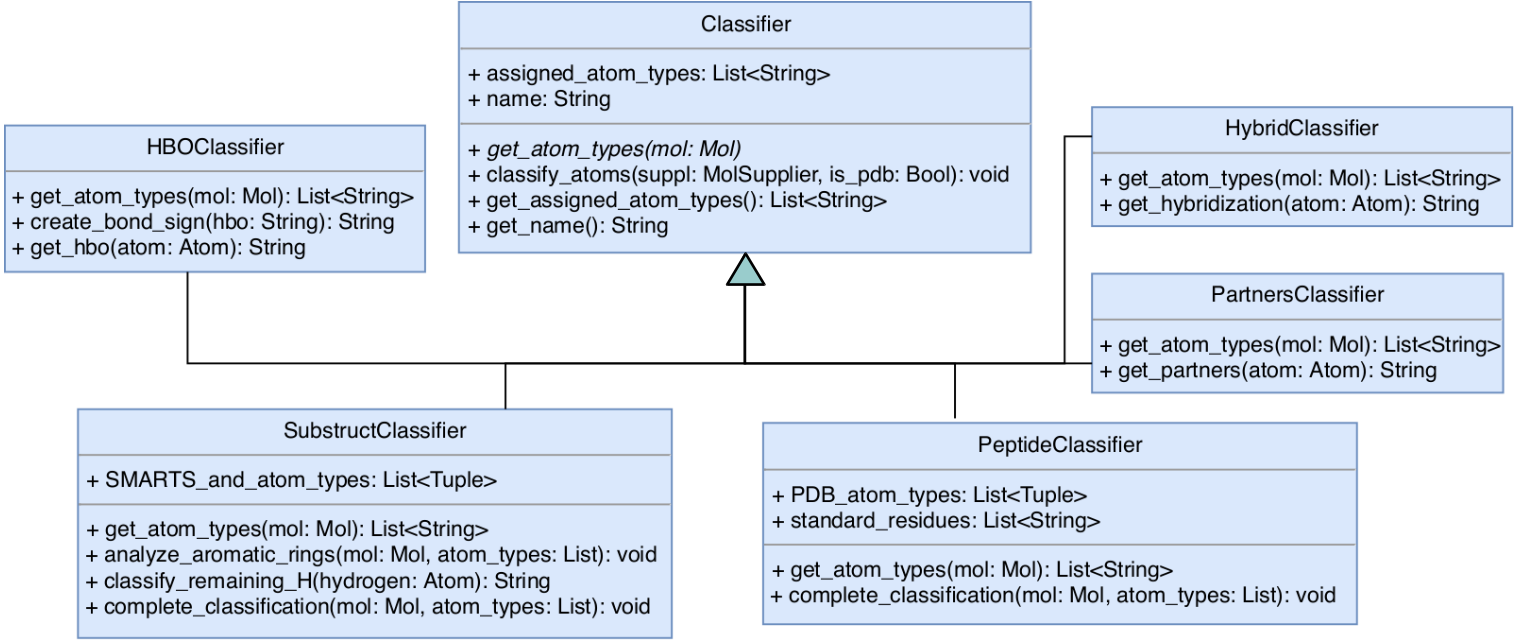
\includegraphics[width=15.1cm]{pictures/diagram_triangle.png}
    \caption{UML diagram tříd popisující třídu Classifier a její podtřídy.}
    \label{classes_UML}
\end{figure}

    
\section{Přiřazení atomových typů}
% \texttt{get\_atom\_types(molecule)}
Každý klasifikátor v adresáři \textbf{\textbackslash classifiers} implementuje abstraktní metodu nadtřídy \verb|get|\\ \verb|_atom_types(molecule)|, která atomům molekuly přiřazuje odpovídající atomové ty\-py. Klasifikátory \verb|hbo|, \verb|hybrid| a \verb|partners| implementují tuto metodu triviálně, neboť využívají příslušné metody tříd Atom a Bond z knihovny RDKit (tab.  \ref{atom_rdkit_methods}). 
%Názvy metod použitých pro klasifikaci jsou uvedeny v tabulce níže.

Pro klasifikátory \verb|substruct| a \verb|peptide| nejsou v třídě Atom v knihovně RDKit implementovány triviální metody, atomy jsou proto těmito klasifikátory klasifikovány pomocí dat z externích souborů. Struktura vytvořených externích souborů a logika  klasifikací je popsána v sekcích \ref{substruct_section} a \ref{peptide_section}. 

\begin{table}[h]
\begin{center}
\label{atom_rdkit_methods}
\renewcommand{\arraystretch}{1.3}
    \begin{small}
    \hspace{7mm}\begin{tabular}{c|l}
        % \hline
        \verb|hbo| & Atom.GetBonds(), Bond.GetBondTypeAsDouble() \\
        \hline
        \verb|hybrid| & Atom.GetHybridization() \\
        \hline
        \verb|partners| & Atom.GetNeighbors() \\
        % \hline
    \end{tabular}
    \end{small}
    \caption{Klíčové metody z knihovny RDKit použité pro přiřazení atomových typů klasifikátory \texttt{hbo}, \texttt{hybrid} a \texttt{partners}.}
\end{center}
\end{table}

\noindent Následující obrázky ilustrují výstup klasifikace atomů molekulu kyseliny karbamové za~použití klasifikátorů \verb|hbo|, \verb|hybrid| a \verb|substruct|.

\begin{figure}[h]
    \centering
    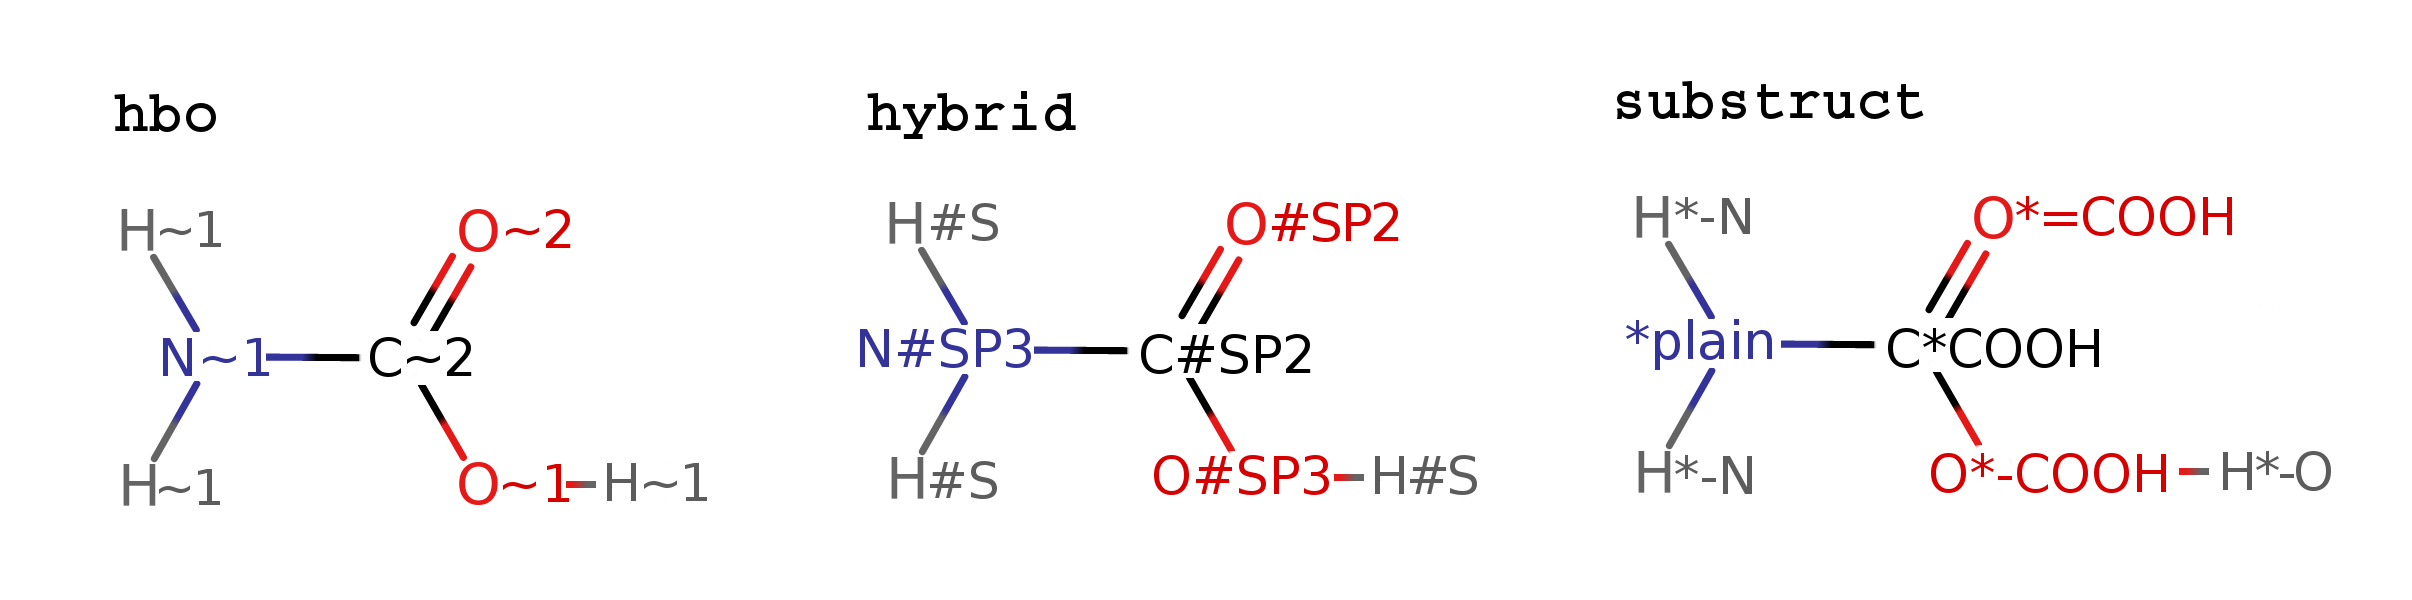
\includegraphics[width=15cm]{pictures/karbamova_merged_popisky.png}
    \caption{Výstupy klasifikací atomů dle klasifikátorů \texttt{hbo}, \texttt{hybrid} a \texttt{substruct}.}
    \label{classfiers_karbamova}
\end{figure}

\subsection{Klasifikátor 'substruct'}
% \texttt{substruct}
\label{substruct_section}
Klasifikátor \verb|substruct| klasifikuje atomy na základě příslušnosti k~charakteristickým strukturním celkům. Byl implementován s cílem reprodukovat atomové typy, které byly úspěšně použity pro parametrizaci empirických metod výpočtu parciálních atomových nábojů \cite{attyp2, attyp1}. 

Strukturní motivy jsou v molekulách detekovány pomocí výrazů SMARTS (kap. \ref{SMARTS}) metodou  \verb|GetSubstructMatches(SMARTS_pattern)|\footnote{Metoda  \texttt{GetSubstructMatches(Chem.MolFromSmarts(SMARTS\_pattern))} je v textu pro názornost syntakticky zjednodušena.} třídy Mol z kni\-hovny RDKit. 
Příkaz \verb|molecule.GetSubstructMatches(SMARTS_pattern)| 
vrací n-tici (\textit{tuple}) n-tic, jež obsahují prvky typu integer. Tato čísla označují atomy molekuly vyhovující danému SMARTS dotazu. Obrázek \ref{h2so5} a kód níže demonstrují užití SMARTS výrazu k vyhledání sulfonové skupiny S(=O)$_2$OH nebo jejích aniontů.

\begin{figure}[h]
    \centering
    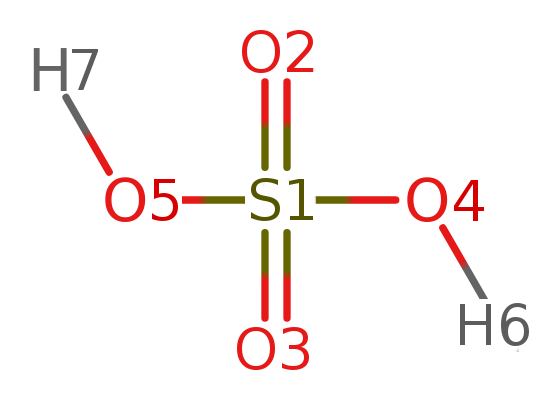
\includegraphics[width=4cm]{pictures/sirovka.png}
    \caption{Molekula kyseliny sírové s číselným označením atomů.}
    \label{h2so5}
\end{figure}

%Čísla atomů vycházejí z pořadí, ve kterém jsou atomy definovány v SDF souboru.


\begin{figure}[H]
\lstset{language=Python, keywordstyle=\color{blue}, basicstyle=\small\ttfamily, commentstyle=\color{orange}, label={smarts_exm}}
% pridat do obrazku vice SMARTSu pro nazornost?
\begin{lstlisting}
>>> SMARTS_pattern = "[SX4](=[OX1])(=[OX1])[OX2,OX1-]"
>>> pattern_atms = molecule.GetSubstructMatches(SMARTS_pattern)
>>> for atom_tuple in pattern_atms:
...    print(atom_tuple, get_elements(atom_tuple))
>>> print(pattern_atms)

Python 3.7.0 (default, Apr 9 2019, 10:31:47)
(1, 2, 3, 4) ('S', 'O', 'O', 'O')
(1, 2, 3, 5) ('S', 'O', 'O', 'O')
((1, 2, 3, 4), (1, 2, 3, 5))
\end{lstlisting}
\caption{Ukázka kódu klasifikátoru \texttt{substruct}. Čísla v n-tici odpovídají atomům molekuly na obrázku \ref{h2so5}.     }
\end{figure}

\bigskip
Pro klasifikaci atomů je klíčovým souborem \textbf{SMARTS\_atom\_types.txt}. Soubor obsahuje SMARTS výrazy, pomocí nichž jsou v molekule hledány strukturní motivy, a~atomové typy, které jsou atomům strukturního motivu explicitně přiřazeny.
Pořadí detekce strukturních motivů odpovídá pořadí SMARTS vstupů v souboru. Některé atomy molekuly mohou příslušet více strukturním motivům, které SMARTS vstupy detekují. Uspořádání SMARTS vstupů v souboru tak ovlivňuje výsledný atomový typ, který je atomu přiřazen. Atomové typy přiřazené jednotlivým atomům lze v souboru předefinovat, stejně jako změnit pořadí SMARTS výrazů, a upravit tak logiku klasifikace a optimalizovat výsledky parametrizace.
\begin{figure}[h]
    \centering
    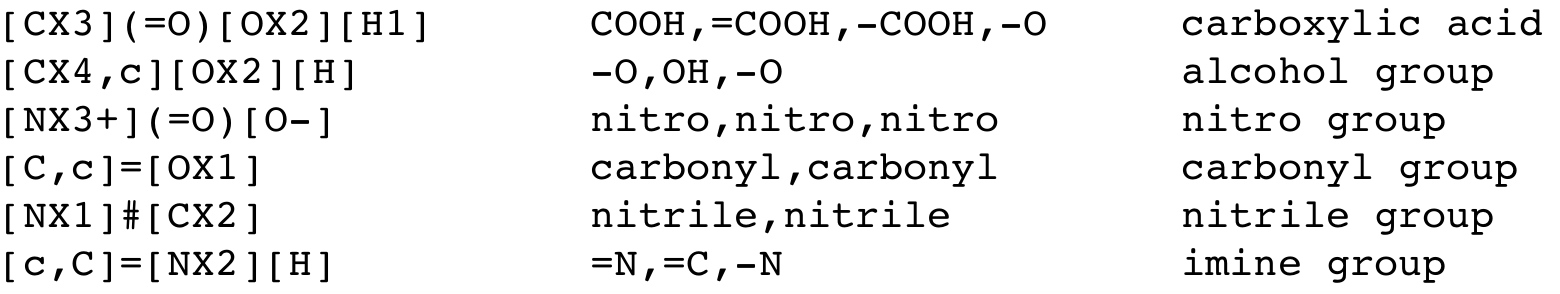
\includegraphics[width=14cm]{pictures/SMARTS_legend_2.png}
    \caption{Struktura souboru \textbf{SMARTS\_atom\_types.txt}. Prostřední sloupec definuje atomové typy atomů dané funkční skupiny.}
    \label{SMARTS_file}
\end{figure}

SMARTS výrazy v souboru \textbf{SMARTS\_atom\_types.txt} byly převzaty ze stránek společnosti Daylight Chemical Information System, Inc. \cite{SMARTS_exm}, pro účely klasifikace atomů však musely být ve většině případů dodatečně upraveny. Vybrané SMARTS výrazy byly rozšířeny o detekci většího počtu atomů nebo byly upraveny tak, aby %se zamezilo redundanci výsledků jednotlivých SMARTS dotazů.
se výsledky jednotlivých SMARTS dotazů nepřekrývaly. 

Úpravu pro snížení redundance výsledků ilustruje následující příklad. Vyhledání karboxylové skupiny za užití výrazu \verb|[CX3](=O)[OX2][H]| je v externím souboru následováno detekcí alkoholové skupiny pomocí výrazu \verb|[CX4,c][OX2][H]|. Pokud by nebyla specifikována vaznost uhlíku ('\verb|CX4|'), vyhledal by daný SMARTS výraz i OH skupiny, které by byly součástí dříve určených karboxylových skupin. 

Rozšíření SMARTS dotazů o detekci více atomů se ve většině případů týkalo detekce vodíků. Pro vyhledání primárních aminů je v uvedeném online zdroji specifikován výraz \verb|[NX3;H2!$(NC=O)]|. Tento výraz byl upraven
na dotaz \verb|[NX3;!\$(NC=O)]([H])[H]|, kterým jsou narozdíl od původního výrazu vodíky již detekovány.
 
\subsection{Klasifikátor 'peptide'}
% \texttt{peptide}
\label{peptide_section}
Klasikace atomů peptidových řetězců přiřazuje atomové typy obdobně na základě příslušnosti atomů ke strukturním celkům. Logika vstupního souboru klasifikátoru \verb|pepti|\\\verb|de| se od struktury externího souboru klasifikátoru \verb|substruct| liší, neboť nepracuje s vyhledáváním strukturních motivů pomocí SMARTS výrazů. 

Symboly atomových typů aminokyselin popsané nomenklaturou IUPAC (CA, CB, HXT, OXT,...) popisují atomy všech proteinogenních residuí. Jednotlivé atomové typy však nijak nereflektují vlastnosti atomů, které popisují, chemická okolí ato\-mů označených stejným atomovým typem se tak často liší (srov. obr. \ref{aa_different_atom_types}). Pro implementaci klasifikátoru \verb|peptide| tak bylo klíčové provést rešerši existujících atomových typů aminokyselin a
%určit napříč všemi aminokyselinami výskyt těchto atomových typů 
každé dvojici 'atomový typ  nomenklatury IUPAC - aminokyselina' přiřadit atomový typ reflektující chemické okolí daného atomu. Navržená klasifikace atomů aminokyselin byla implementována s cílem reprodukovat atomové typy, které byly použity pro úspěšnou parametrizaci empirických metod \cite{GDAC, attyp_peptides}.

\begin{figure}[H]
\label{aa_different_atom_types}
\begin{center}
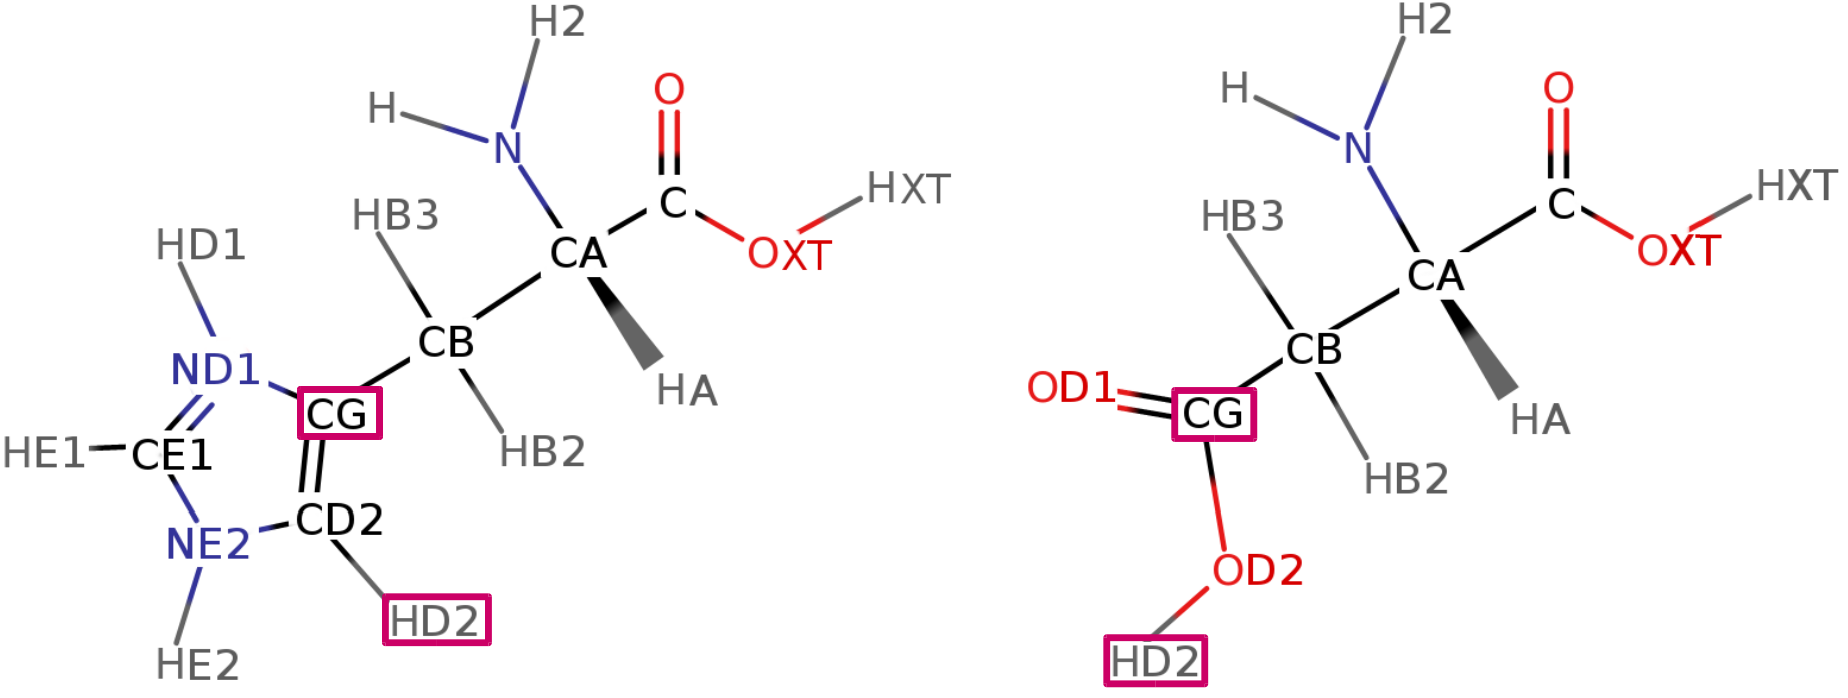
\includegraphics[width=13.5cm]{pictures/asp_his_merged_squares.png}
\caption{Strukturní vzorce histidinu a kyseliny asparagové s atomovými typy nomenklatury IUPAC verze 3.0. Atomy CG a HD2 jsou v molekulách součástí odlišných strukturních celků, je tedy vhodné každému z nich přiřadit jiný atomový typ.}
\end{center}
\end{figure}

% vložit ilustrační obrázek souboru PDB_atom_types.txt?

% dát Krabíkovi vědět, že dokumentaci a štábní kulturu budu dělat až o víkendu před 13. květnem - aby s tím počítal a měl v pondělí a v úterý čas na to, aby mi to zkontroloval
% 15. května ráno nejpozději nahrávám na IS a jedu na kampus odevzdat


 



